\subsection{CFD results}
\label{subsec:cfd_results}

The simulation was run for $100$ iterations, which was enough to reach a good level of convergence considering the residuals and a converged value of the drag coefficient.

In particular, the final value of the drag coefficient was computed as $C_d = 0.86$.
This value is generally considered as almost out of the range of the drag coefficient for a rocket, which is usually between $0.7$ and $0.8$.
However, given the shape of the rocket and in particular the four fins that have a considerable impact on the drag coefficient, this value can be considered reasonable\footnote{We have runned multiple simulation varying of some perceptual point the velocity at the inlet, and we notice that the drag coefficient was extremely affected. We believe that this has something to do with an error in the simulation setup rather than a physical phenomenon.}.

\begin{figure}[H]
    \centering
    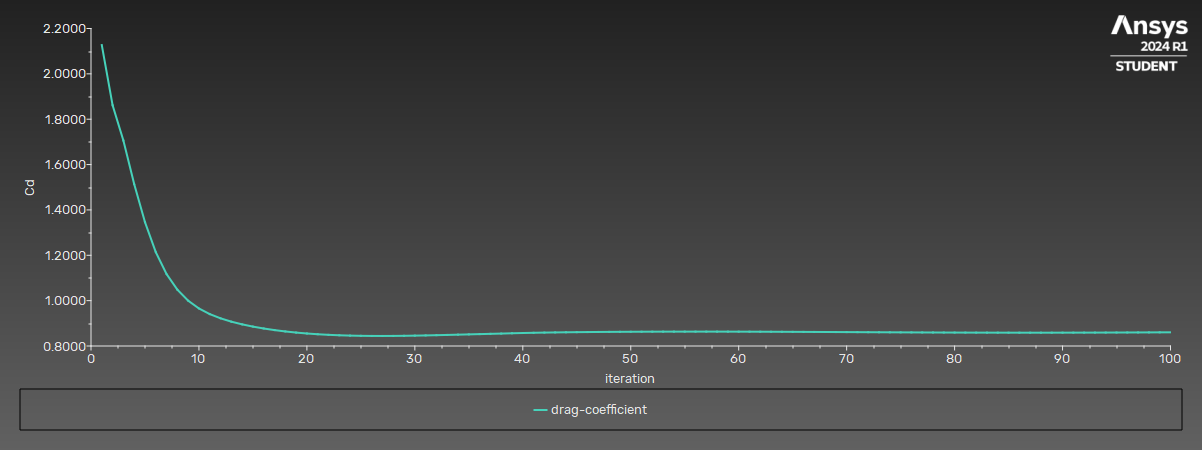
\includegraphics[width=.8\textwidth]{img/Results/Drag_coefficient_plot.png}
    \caption{Drag coefficient as function of the number of iterations.}
    \label{fig:drag_coefficient}
\end{figure}

\begin{figure}[H]
    \centering
    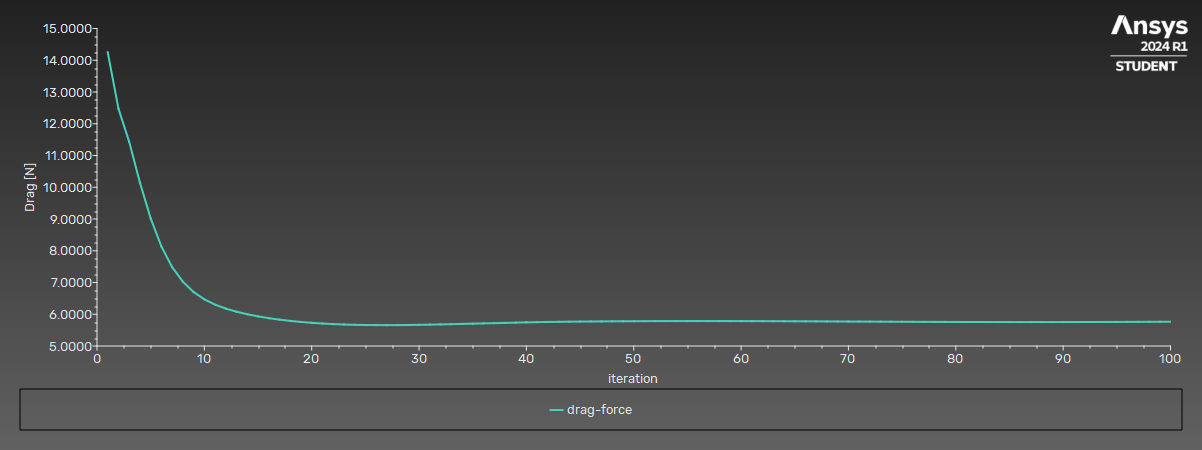
\includegraphics[width=.8\textwidth]{img/Results/Drag_force.png}
    \caption{Drag force as function of the number of iterations.}
    \label{fig:drag_force}
\end{figure}

\begin{figure}[H]
    \centering
    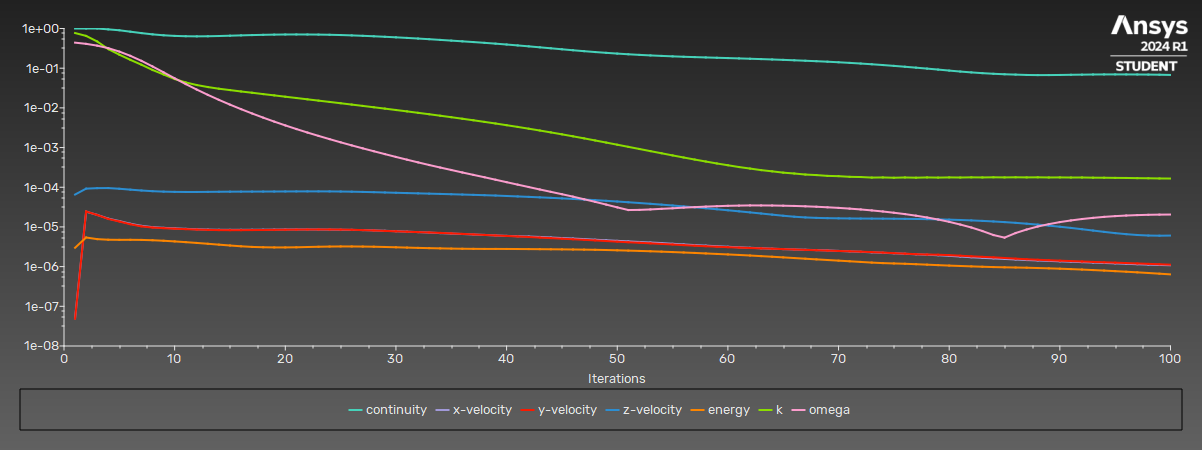
\includegraphics[width=.8\textwidth]{img/Results/Residuals_plot.png}
    \caption{Residuals as function of the number of iterations.}
    \label{fig:residuals}
\end{figure}


\subsubsection{Result visualization}
\label{subsubsec:result_visualization}

Although the main focus of the study was to compute the drag coefficient of the rocket, we can also proceed to analyze the pressure and velocity field around the rocket which can give us some insights on the flow field.

\paragraph{Pressure field}

Pressure contours around the rocket are shown in Figures \ref{fig:pressure_field} and \ref{fig:pressure_field_nose}.

\begin{figure}[H]
    \centering
    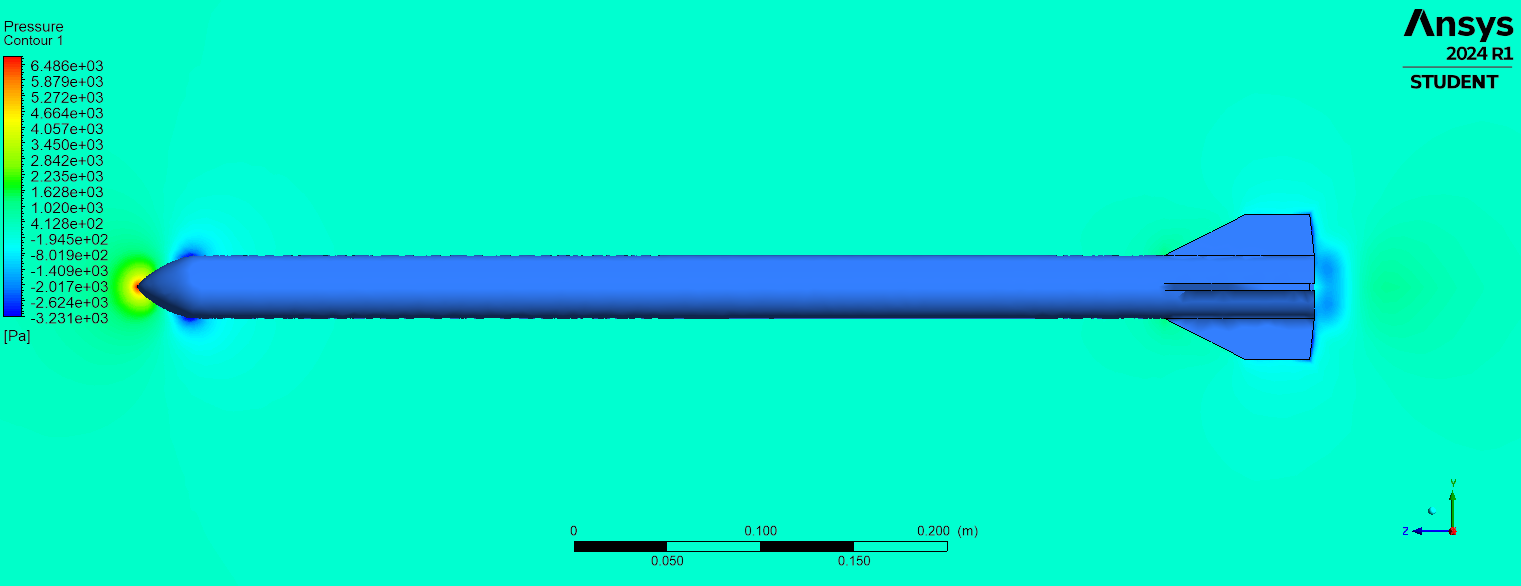
\includegraphics[width=.8\textwidth]{img/Results/Coutours_Pressure.png}
    \caption{Pressure contours around the rocket. Expected behavior is observed, with the pressure maximum at the bottom of the nose cone and the minimum at both the top of the nose cone. In the rear of the rocket, a low pressure area is formed even if not very pronounced.}
    \label{fig:pressure_field}
\end{figure}

\begin{figure}[H]
    \centering
    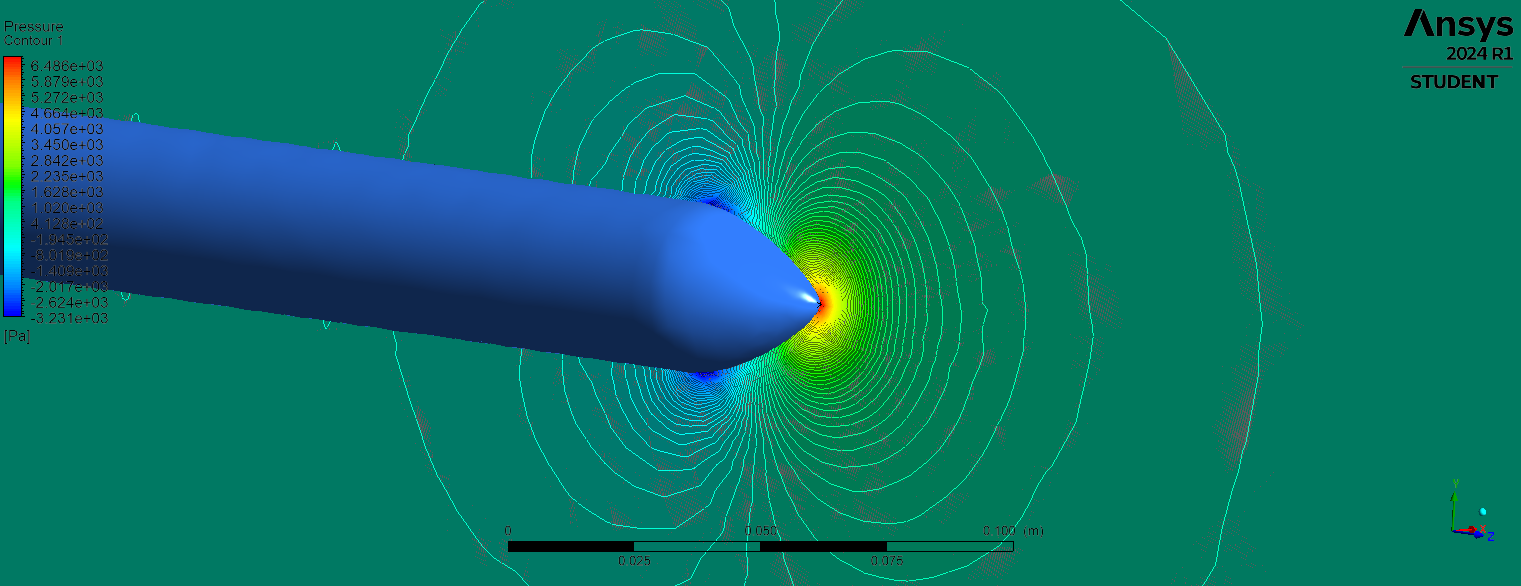
\includegraphics[width=.8\textwidth]{img/Results/Contours_Pressure_Nose.png}
    \caption{Detail of the pressure field around the nose cone.}
    \label{fig:pressure_field_nose}
\end{figure}


\paragraph{Velocity field}

Velocity contours and streamlines around the rocket are shown in Figures \ref{fig:velocity_field}, \ref{fig:velocity_field_nose} and \ref{fig:streamline_lateral}.

\begin{figure}[H]
    \centering
    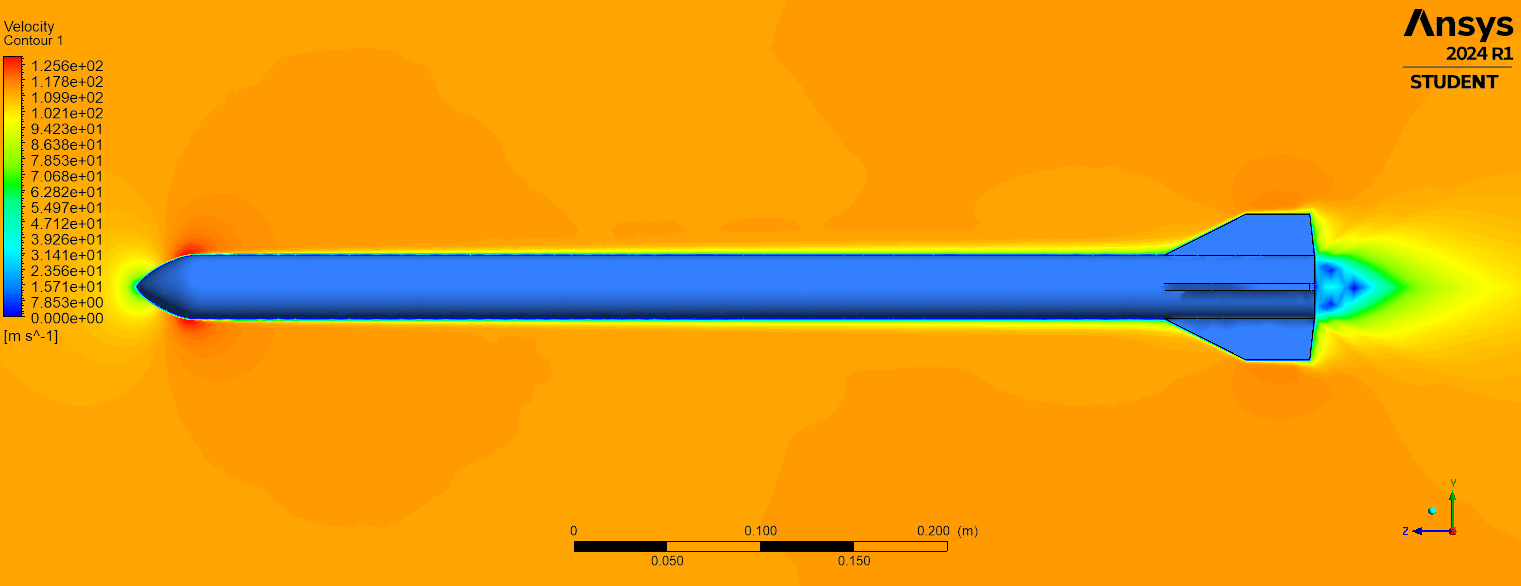
\includegraphics[width=.8\textwidth]{img/Results/Coutours_Velocity.png}
    \caption{Velocity contours around the rocket. Expected behavior is observed, with the velocity maximum at the bottom of the nose cone and the minimum at both the top of the nose cone and the rear of the rocket. No-slip condition are also respected.}
    \label{fig:velocity_field}
\end{figure}

\begin{figure}[H]
    \centering
    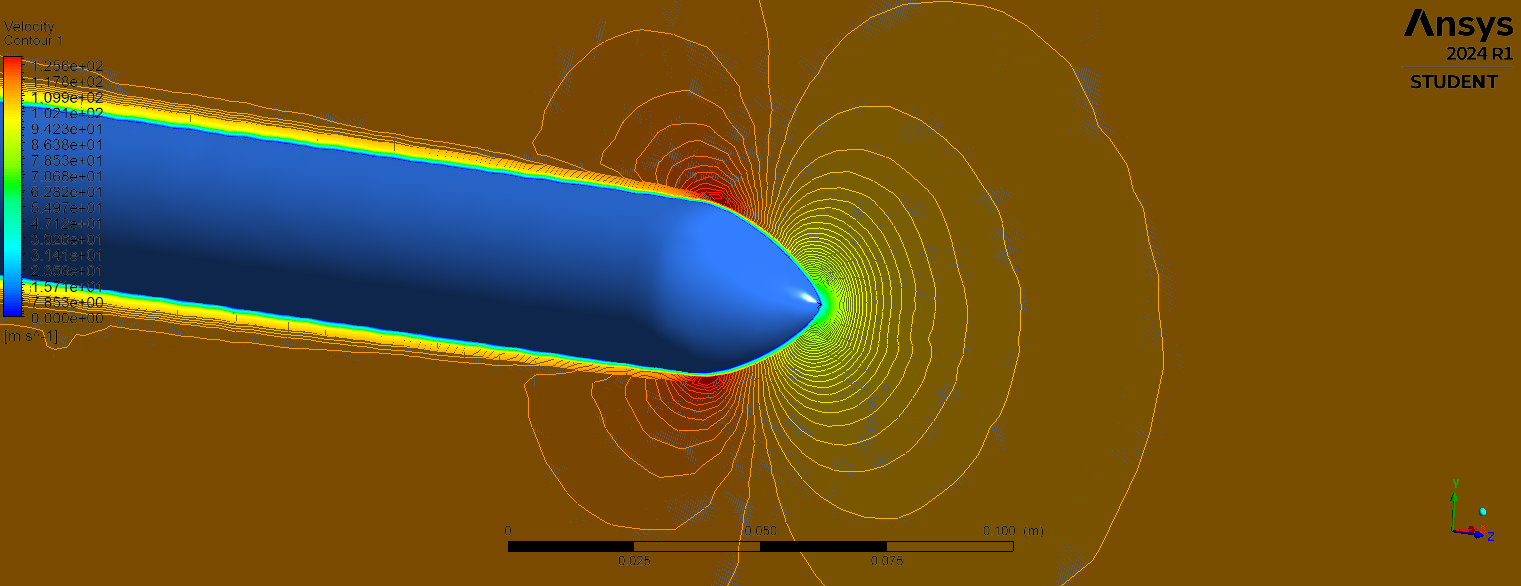
\includegraphics[width=.8\textwidth]{img/Results/Contours_Velocity_Nose.png}
    \caption{Detail of the velocity field around the nose cone.}
    \label{fig:velocity_field_nose}
\end{figure}

\begin{figure}[H]
    \centering
    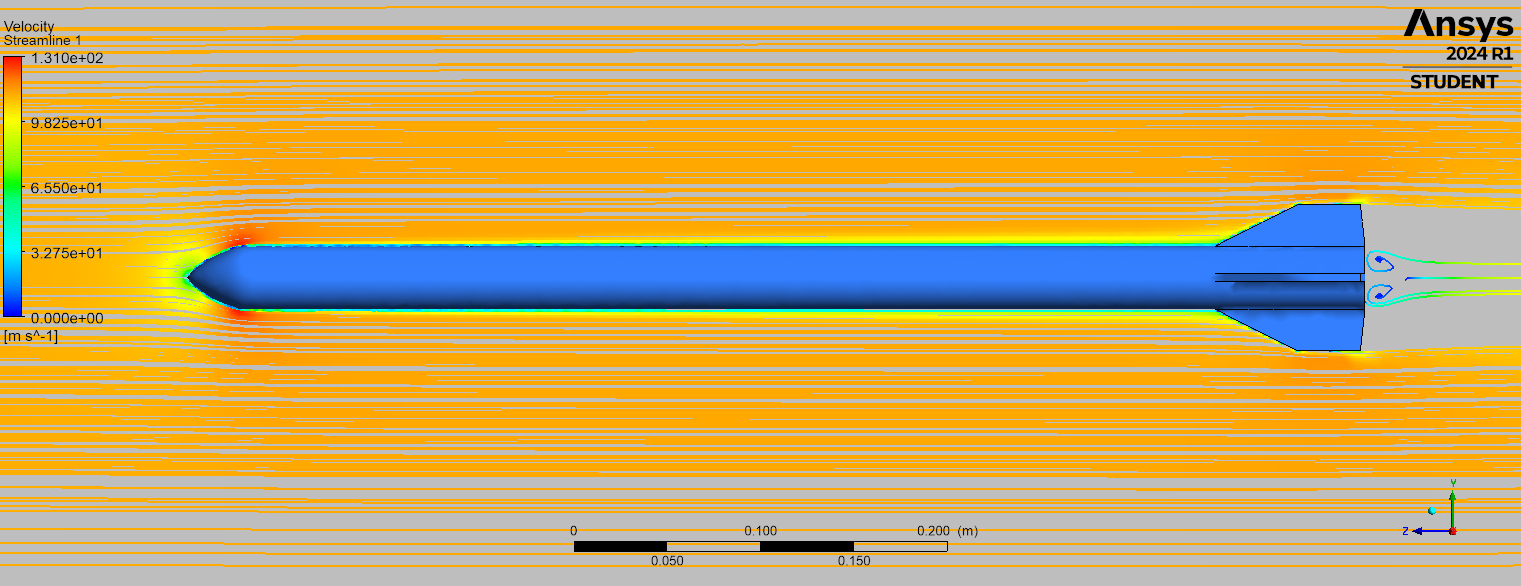
\includegraphics[width=.8\textwidth]{img/Results/Streamline_lateral.png}
    \caption{Streamlines around the rocket.}
    \label{fig:streamline_lateral}
\end{figure}


\paragraph{Vorticity field}

Vorticity streamlines are highlighted in Figure \ref{fig:vorticity_field}.

\begin{figure}[H]
    \centering
    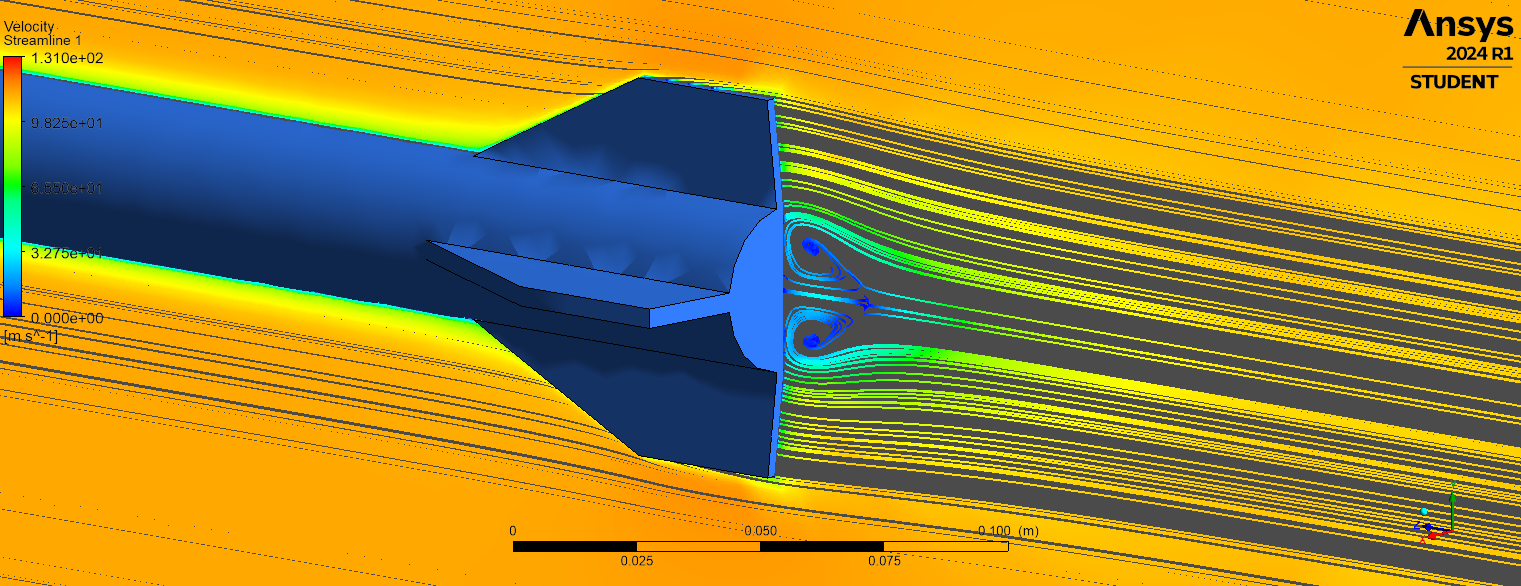
\includegraphics[width=.8\textwidth]{img/Results/Streamline_Fins.png}
    \caption{Vortex shedding behind the rocket are clearly visible.}
    \label{fig:vorticity_field}
\end{figure}


\paragraph{Temperature field}

Temperature contours around the rocket are shown in Figure \ref{fig:temperature_field}.

\begin{figure}[H]
    \centering
    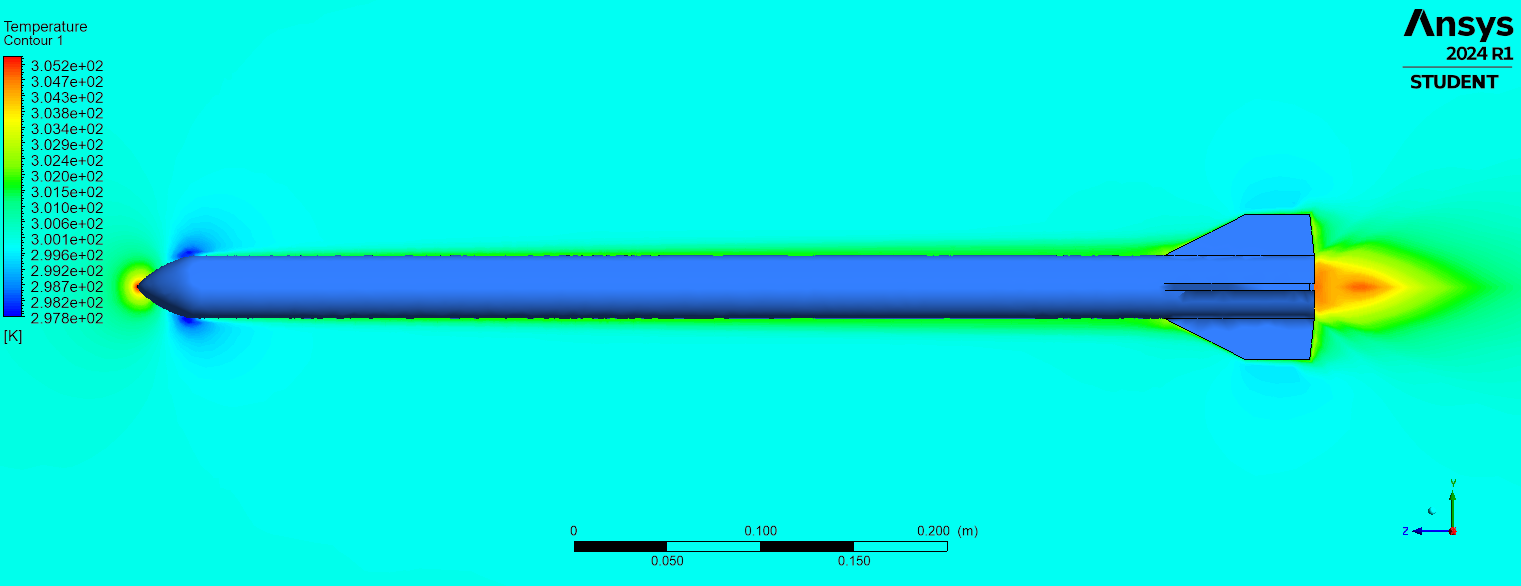
\includegraphics[width=.8\textwidth]{img/Results/Coutours_Temperature.png}
    \caption{Temperature field around the rocket. The variation is minimal ($+5 ^\circ C$ at the nose and $-2 ^\circ C$ at the first full cross-section of the body). It's interesting to see that the temperature rises also at the rear, where a vortex are formed.}
    \label{fig:temperature_field}
\end{figure}